% =====================================================================
% Paper 1 — NegoPlay
% "From Bridge Tables to the Negotiation Table"
% Target: Springer edited book
%   "Recent Advances on Scientific Computing, AI and Other Software Tools"
%   (papers collected from the Jyväskylä conference in honour of
%    Prof. Olivier Pironneau's 80th birthday, org. P. Neittaanmäki)
%
% NOTE ON FORMAT: drafted in the standard `article` class. Once the
% volume's official template arrives (likely Springer svmult), the
% content ports section-by-section with no structural change.
%
% Build:  xelatex negoplay_paper1.tex  (run 2-3x for refs)
% =====================================================================
\documentclass[11pt,a4paper]{article}

\usepackage[margin=2.6cm]{geometry}
\usepackage{graphicx}
\usepackage{booktabs}
\usepackage{array}
\usepackage{amsmath,amssymb}
\usepackage{xcolor}
\usepackage{caption}
\usepackage{enumitem}
\usepackage[colorlinks=true, linkcolor={navy}, citecolor={navy}, urlcolor={steel}]{hyperref}

\definecolor{navy}{HTML}{16324F}
\definecolor{steel}{HTML}{2C5F8A}

\graphicspath{{../../docs/images/}}
\captionsetup{font=small, labelfont={bf,color=navy}}

\newcommand{\rhoS}{\rho_{\mathrm{S}}}

\title{\color{navy}\textbf{From Bridge Tables to the Negotiation Table:\\
Cross-Domain Behavioral Consistency of\\ Game-Derived Decision-Making Profiles}}

\author{Anna Ben-Shushan\\[2pt]
\small LUT School of Engineering Sciences, LUT University, Lappeenranta, Finland\\
\small \texttt{anna.ben.shushan@student.lut.fi}}

\date{\small Draft, September 2026 \\[2pt]
\footnotesize Prepared for the Springer OP80 volume
\emph{Recent Advances on Scientific Computing, AI, and Other Software Tools}}

\begin{document}
\maketitle

% ------------------------------------------------------------------
\begin{abstract}
\noindent
Business negotiation is one of the most consequential forms of
decision-making under uncertainty, yet it is difficult to study
empirically: real negotiations are private, and no public dataset links
how a person makes decisions in general to how they negotiate. We
propose contract bridge as a measurable laboratory. Bridge bidding is a
structured sequence of decisions under incomplete information in which
every action is recorded and scored, and the same player is observed
across hundreds of comparable decision problems. From 149{,}208
board-level records of five European championships (2016--2025) we show,
first, that elite players form a statistical \emph{continuum} of styles
rather than discrete clusters (silhouette $\le 0.24$; HDBSCAN detects
zero clusters across five preprocessing configurations). We therefore
profile the \emph{tails} of this continuum with a percentile rule gated
by a one-sided binomial significance test, obtaining four behaviorally
distinct extreme profiles plus a Generalist baseline (Cohen's $d$
between $2.13$ and $4.62$, all $p<0.05$). A large language model then
reads a fixed-seed sample of each profiled player's raw deals (the
cards held, the full auction, and the result), directed to the
profile's defining behavioral axis but never shown the engineered
feature values, and extracts observable skills with deal-level
evidence, from which we build profile-conditioned agents. The agents play both bridge and simulated
multi-round business negotiations against fixed, rule-based
counterparts. The negotiation counterpart is calibrated on 5{,}247
human--human bargaining dialogues grounded in real Craigslist listings.
Whether a profile \emph{wins} in both
domains proves weak and metric-sensitive (Spearman
$\rhoS \approx +0.2$ to $+0.5$). Whether a profile \emph{behaves
consistently} across domains is strong: bridge-side aggression and
negotiation-side demand depth (how far below the asking price an agent
pushes its offers) align at $\rhoS = +0.80$, and an inverse-prompt control
that swaps the extracted skills between the profiles flips the
correlation to $\rhoS = -0.90$, showing the transfer is carried by the
game-derived skills rather than by the profile label.
All thresholds, prompts, seeds, and outputs are released for full
reproducibility. The results are an indication ($K=5$ profiles), not a
proof; they establish a validated, reproducible pipeline for studying
cross-domain transfer of decision-making styles.
\end{abstract}

\vspace{0.5em}
\noindent\textbf{Keywords:} decision-making under uncertainty; contract
bridge; negotiation; large language model agents; behavioral profiling;
cross-domain transfer; reproducibility.

% ==================================================================
\section{Introduction}\label{sec:intro}

Negotiation, over prices, alliances, contracts, and platforms, is a
sequence of decisions under uncertainty with conflicting objectives:
demand more and risk the deal, or concede and lose surplus. Despite its
economic weight, negotiation behavior is hard to study at the level of
the \emph{individual decision-maker}. Real negotiations are private and
rarely recorded; the transcripts that are public (teaching cases,
mediation examples) are edited and anonymized; and, most importantly, no
public dataset links the \emph{same person's} general decision-making
style to their observed negotiation behavior.

Contract bridge offers a way around this measurement problem. Bridge
bidding is a formal negotiation-like protocol: partners exchange
information through a constrained language of bids while opponents
contest the auction, all under incomplete information (each player sees
only 13 of 52 cards). Unlike real negotiations, \emph{every} decision is
recorded, timestamped to a specific deal, and objectively scored, and
elite players are observed over hundreds of comparable decision
problems. Bridge has long served as a benchmark for AI under imperfect
information \cite{ginsberg2001gib,rong2019bridge}; here we use it
differently: not to play bridge well, but as a \emph{measurable
laboratory of individual decision-making style}.

This paper asks a single question:

\begin{quote}
\emph{If we derive a player's decision-making profile from their real
bridge record and instantiate it as an autonomous agent, does the
profile's behavioral signature persist when the agent negotiates in a
business setting?}
\end{quote}

We answer it with a four-stage pipeline (Fig.~\ref{fig:radar} through
Fig.~\ref{fig:control}) and report both a positive result and an
instructive negative one.

\paragraph{Contributions.}
\begin{enumerate}
  \item \textbf{A continuum, not clusters.} Across five escalating
  preprocessing configurations and three algorithm families (K-Means,
  Gaussian mixtures, HDBSCAN), elite championship players show no
  discrete cluster structure (Sec.~\ref{sec:continuum}). This negative
  result redirects the methodology and is, to our knowledge, the first
  systematic demonstration of style-space continuity at championship
  level.
  \item \textbf{Statistically gated tail profiling.} We profile
  the \emph{tails} of the continuum: a player is assigned to a profile
  only if they are in the top decile of the profile's defining axis
  \emph{and} a one-sided binomial test rejects the population baseline
  at $p<0.05$ (Sec.~\ref{sec:profiles}). We document how expert review
  exposed a small-sample artefact in our first version and how the gate
  repairs it: a reusable recipe for rare-event behavioral profiling.
  \item \textbf{Evidence-grounded skill extraction.} A large
  language model (LLM) reads a seeded sample of each profiled player's
  raw deals (cards, auction, result) and writes observable skills with
  per-deal evidence citations. The LLM is directed to the profile's
  defining behavioral axis but never shown the engineered feature
  values or any comparative statistics, so every skill must be
  verifiable from the cited deals (Sec.~\ref{sec:stage2}); whether
  downstream behavior follows the skill \emph{content} rather than the
  profile identity is then tested, not assumed, by the inverse-prompt
  control.
  \item \textbf{A validated cross-domain testbed.} Profile-conditioned
  agents play bridge and negotiate against \emph{fixed} rule-based
  counterparts. The bridge metric is validated with a zero-intelligence
  baseline \cite{gode1993zi} and a double-dummy reference
  \cite{ginsberg2001gib}; the negotiation counterpart is calibrated on
  5{,}247 real negotiations \cite{he2018decoupling}
  (Sec.~\ref{sec:stage4}).
  \item \textbf{Principal findings.} Decision \emph{style} transfers
  strongly (behavioral alignment $\rhoS=+0.80$), and an inverse-prompt
  control flips it to $\rhoS=-0.90$, demonstrating skill-mediated
  transfer. Whether a style \emph{wins} in both domains is weak and
  metric-dependent ($\rhoS\approx+0.2$ to $+0.5$): winning depends on
  the opponent and payoff structure, behaving does not
  (Sec.~\ref{sec:results}).
\end{enumerate}

Throughout, we adhere to two methodological principles: every
experimental condition needed to reproduce the study is stated
explicitly (the Reproducibility Statement and
Appendix~\ref{app:protocol} map each reported number to a runnable
script), and evaluation scenarios are ordered from \emph{trivial}, where
the reader can predict which profile should prevail and so builds trust
in the instrument, to non-trivial.

% ==================================================================
\section{Related Work}\label{sec:related}

\paragraph{Bridge as an AI benchmark.} Ginsberg's GIB introduced
double-dummy analysis as an objective reference for bridge decisions
\cite{ginsberg2001gib}; Rong et al.\ trained estimation and policy
networks for competitive bidding on $\sim$1M deals
\cite{rong2019bridge}. These works optimize \emph{play strength}; we
instead treat the human record as behavioral data.

\paragraph{Games, negotiation, and agents.} Self-play systems master
perfect-information games \cite{silver2018general}; Diplomacy work
combines language and strategic reasoning and studies honesty and
sanctioning in negotiation-like play
\cite{kramar2022negotiation,bakhtin2022cicero}. End-to-end negotiation
dialogue agents were introduced by Lewis et al.\
\cite{lewis2017deal}; He et al.\ decoupled strategy from generation and
released the Craigslist Bargaining corpus we use for calibration
\cite{he2018decoupling}. Human negotiation corpora with per-participant
trait measures now exist, notably CaSiNo, a multi-issue corpus with
Big-Five and social-value-orientation scores per negotiator
\cite{chawla2021casino}. For LLM negotiators, NegotiationArena
benchmarks multi-turn agent-vs-agent bargaining and shows that injected
behavioral tactics measurably shift payoffs
\cite{bianchi2024negotiationarena}; Abdelnabi et al.\ contribute
multi-party, multi-issue scorable negotiation games
\cite{abdelnabi2024cooperation}; and a 180{,}000-negotiation
competition finds that prompted \emph{warmth} and \emph{dominance}
systematically shape outcomes \cite{vaccaro2026advancing}, independent evidence that prompt-carried style becomes bargaining
behavior. Our contribution is orthogonal to all of these: we do not
train or benchmark a negotiator; we test whether a profile derived from
\emph{real cross-domain human data} persists in another domain.

\paragraph{Zero-intelligence baselines.} Gode and Sunder showed that
budget-constrained random traders (``ZI-C'') achieve high allocative
efficiency, making them the canonical null model for market behavior
\cite{gode1993zi}. We adopt a ZI-C bidder as the falsification baseline
for our bridge skill metric: any metric a constrained random agent can
top is measuring structure, not skill.

\paragraph{Styles, archetypes, and behavioral economics.} Archetypal
analysis represents data by its extreme points rather than central
prototypes \cite{cutler1994archetypal}; our tail profiling is related in
spirit but operates on individual, interpretable behavioral axes with an
explicit significance gate, rather than fitting a convex-combination
factorization. Prospect theory motivates why payoff structure shapes
risk appetite \cite{kahneman1979prospect}, and coopetition frames the
simultaneous cooperation/competition that bridge partnerships embody
\cite{brandenburger1996coopetition}. Classical negotiation analysis
provides the surplus-splitting lens
\cite{raiffa1982art,nash1950bargaining}.

\paragraph{Cross-situational consistency of style.} Whether behavioral
dispositions persist across situations is a classical question in
personality psychology: consistency emerges reliably only when behavior
is \emph{aggregated} over many observations \cite{epstein1979stability},
and stable dispositional signatures coexist with systematic situational
variation \cite{mischel1995cognitive}. For risk attitude specifically,
human self-report evidence indicates substantial domain-specificity
\cite{weber2002domain}. These findings calibrate the scope of our claim:
we measure the cross-domain consistency of \emph{profile-conditioned
agents}; whether the same consistency holds for the underlying human
players is a distinct, open question left for future work with
trait-annotated human negotiation data (Sec.~\ref{sec:conclusion}).

\paragraph{LLMs as behavioral simulacra.} LLMs conditioned on personas
can reproduce human-like behavioral distributions
\cite{park2023generative,argyle2023out,aher2023using}. Two validity
risks are documented. The first is \emph{tautology}: an agent told it
is aggressive will act aggressively. The second is the converse, \emph{non-enactment}: role-playing agents can state a persona's beliefs
yet fail to behave accordingly \cite{mannekote2025roleplaying}, so
persona conditioning cannot simply be assumed to work. Our design
answers both empirically: skills are extracted from raw hands under a
deal-level evidence requirement (Sec.~\ref{sec:stage2}), and an
inverse-prompt control swaps
skills between identities and measures whether behavior follows
(Sec.~\ref{sec:control}), precisely the belief-vs-behavior
consistency check this literature calls for.

% ==================================================================
\section{Data}\label{sec:data}

We scraped the public tournament archive of the European Bridge League
(EBL) for five championships. Each record is one board (deal) in one
room, with identity, deal, auction, and result fields. The corpus
contains \textbf{149{,}208 board-room records} ($\times$48 columns) and
$\sim$2{,}500 named players.

\begin{table}[h]
\centering\small
\caption{Corpus composition and field coverage per championship.}
\label{tab:data}
\begin{tabular}{lrccc}
\toprule
Championship & Rows & Player names & Card holdings & Bidding sequences\\
\midrule
Budapest 2016 & 38{,}240 & 100\% & 56\% & 0\%\\
Ostend 2018   & 32{,}384 & 100\% & 53\% & 0\%\\
Madeira 2022  & 32{,}256 & 100\% & 51\% & 0\%\\
Herning 2024  & 34{,}048 & 100\% & 56\% & 100\%\\
Poznan 2025   & 12{,}280 & 100\% & 51\% & 100\%\\
\midrule
Total & 149{,}208 & 99.9\% & 54\% & 31\% (46{,}230 sequences)\\
\bottomrule
\end{tabular}
\end{table}

Older EBL microsites do not expose machine-readable auctions, so
bidding-dependent features use the 46{,}230 rows (31\%,
Table~\ref{tab:data}) of Herning~2024 and Poznan~2025, while
contract/outcome features use all 149K rows. Each
board is played in two rooms by different pairs, the duplicate
structure that later yields an opponent-controlled skill metric
(Sec.~\ref{sec:bridgemetric}). All data are public tournament records of
named professional players published by the EBL; we collect no private
or demographic information.

% ==================================================================
\section{Stage 1: Discovering Decision-Making Profiles}\label{sec:stage1}

\subsection{Behavioral features}\label{sec:features}

For every player we compute per-player rates from two complementary
families: \emph{outcome} features, derived from the final contract the
player declared (what they committed to), and \emph{process} features,
derived from their calls inside the auction (how they got there). A
player enters the analysis only with $n_{\mathrm{declared}}\ge 50$
declared boards \emph{and} $n_{\mathrm{bidding}}\ge 50$ boards with
auction data, leaving \textbf{563 qualifying players}. Interpreting
per-player rates only after aggregating $\ge 50$ observations follows
the aggregation principle of behavioral-stability research
\cite{epstein1979stability}: single-situation behavior is noisy, but
aggregated tendencies are stable.

\begin{table}[h]
\centering\small
\caption{Behavioral features. Family A is computed on declarer boards
(all 149K rows); Family B on any seat from full auctions (46K rows).
Features with coefficient of variation $\mathrm{cv}<0.10$ across players
(e.g.\ mean contract level, calls per board) carry almost no
between-player signal and are excluded from structure analysis.}
\label{tab:features}
\begin{tabular}{llp{7.3cm}}
\toprule
Family & Feature & Definition (per-player rate)\\
\midrule
A (outcome) & \texttt{slam\_rate}      & declared contracts at level 6--7\\
A & \texttt{partscore\_rate} & declared contracts at levels 1--3 (safe stops)\\
A & \texttt{nt\_rate}        & declared contracts in no-trump\\
A & \texttt{double\_rate}    & own declared contracts doubled by opponents\\
\midrule
B (process) & \texttt{opening\_rate}      & boards where the player opened the auction\\
B & \texttt{preempt\_rate}       & openings at level $\ge 2$ (obstructive)\\
B & \texttt{intervention\_rate}  & entries into the opponents' auction\\
B & \texttt{penalty\_double\_rate} & boards where the player doubled the
opponents\footnotemark\\
\bottomrule
\end{tabular}
\end{table}
\footnotetext{The feature counts all doubles (takeout and penalty
alike); both are an active choice to contest the auction, so it measures
\emph{aggressive doubling}. We keep the historical column name for
reproducibility.}

Note the asymmetry: \texttt{double\_rate} is partly
opponent-dependent (being doubled requires the opponents' decision) and
is therefore \emph{not} used as a profile-defining axis below; all four
defining axes are the player's own actions.

\subsection{Finding 1: a continuum, not clusters}\label{sec:continuum}

To ensure that the absence of cluster structure is not an artefact of
inadequate preprocessing, we ran a five-configuration audit before
accepting any negative result: (V1) StandardScaler only; (V2)
StandardScaler + PCA(3) \cite{jolliffe2002principal}; (V3a--c)
RobustScaler + cv-filter + correlation pruning + Mahalanobis outlier
removal ($\alpha=0.01$) + PCA(5), feeding K-Means \cite{lloyd1982least},
a Gaussian mixture with BIC selection \cite{schwarz1978estimating}, and
HDBSCAN.

\begin{table}[h]
\centering\small
\caption{Cluster-structure audit. Silhouette follows
Rousseeuw \cite{rousseeuw1987silhouettes}; HDBSCAN follows
\cite{campello2013density}.}
\label{tab:audit}
\begin{tabular}{llccc}
\toprule
Config & Algorithm & Best $k$ & Silhouette & HDBSCAN clusters\\
\midrule
V1 & K-Means & 4 & $\sim$0.15 & 0\\
V2 & K-Means (PCA 3) & 4 & \textbf{0.24} & 0\\
V3a & K-Means (full prep.) & 2 & 0.17 & n/a\\
V3b & GMM + BIC & 2 & 0.14 & n/a\\
V3c & HDBSCAN & n/a & n/a & \textbf{0}\\
\bottomrule
\end{tabular}
\end{table}

Three observations converge. First, silhouette never exceeds $0.24$
(values near $0$ mean points sit on cluster boundaries). Second, the
density-based HDBSCAN, free of K-Means' convexity assumptions, labels \emph{all} 563 players as noise in every configuration. Third,
\emph{more} aggressive preprocessing makes separation \emph{worse}
(V2$\to$V3a: $0.24\to0.17$): outlier removal deletes precisely the
extreme players who carry the weak signal. The PCA spectrum decays
gradually (PC1 $=24.6\%$, PC2 $=19.1\%$, PC3 $=13.5\%$, \ldots) with no
dominant component, the signature of a smooth distribution. We
conclude that elite championship players occupy a \textbf{continuum} of
styles, consistent with expertise research on maximal adaptation to task
constraints among top performers \cite{ericsson1996expert}. Partitioning
such data is the wrong operation; profiling its \emph{tails} is not.

\subsection{Extreme-percentile profiling with a significance gate}\label{sec:profiles}

Let $x_{a}(i)$ be player $i$'s rate on defining axis $a$, with
population mean $\mu_a$, standard deviation $s_a$, and z-score
$z_a(i) = (x_a(i)-\mu_a)/s_a$. The four defining axes and their
profiles are: \texttt{slam\_rate} $\to$ \emph{Slam Hunter},
\texttt{partscore\_rate} $\to$ \emph{Insurance Player},
\texttt{penalty\_double\_rate} $\to$ \emph{Fighter}, and
\texttt{nt\_rate} $\to$ \emph{NT Specialist}. Player $i$ is assigned to
profile $a^{*} = \arg\max_a z_a(i)$ iff both gates hold:
\begin{equation}
z_{a^{*}}(i) \;\ge\; Q_{0.90}\bigl(z_{a^{*}}\bigr)
\qquad\text{and}\qquad
\Pr\bigl[X \ge k_i \,\big|\, X\sim\mathrm{Bin}(n_i, \mu_{a^{*}})\bigr] < 0.05,
\label{eq:gate}
\end{equation}
where $k_i$ is the player's raw event count and $n_i$ the relevant
denominator (declared boards for Family A axes; bidding boards for the
Fighter axis). Players failing either gate are \emph{Generalists}, retained as the elite baseline, not discarded. Profile names are
human-chosen domain labels for ``extreme on axis $a$''; nothing
downstream depends on the name (Sec.~\ref{sec:control} tests this).

\paragraph{Why the binomial gate exists: an expert-review episode.}
Our first release (v2.0) used $n_{\mathrm{declared}}\ge20$ and the
percentile gate alone, yielding 807 players and 64 Slam Hunters with a
mean slam rate $2.8\times$ baseline. Expert review by a national-level
bridge player flagged a rare-event artefact: with a
$\sim$4--6\% slam baseline, a player with 20 boards and 2 slams shows a
10\% rate whose exact 95\% confidence interval, $[1.2\%,\,31.7\%]$
(Clopper--Pearson \cite{clopper1934use}), is indistinguishable from
the baseline. Indeed 41\% of v2.0 ``Slam Hunters'' had fewer than 30
declared boards. Version 2.1 raised the floor to 50 boards and added the
binomial gate of Eq.~\eqref{eq:gate}: the cohort shrinks to 20 Slam
Hunters whose median $n_{\mathrm{declared}}$ jumps from 42 to
\textbf{216} and whose CI, $[6.3\%, 15.2\%]$, clears the baseline.
Effect ratios become more conservative (e.g.\ $2.8\times\to1.84\times$), but every surviving assignment is statistically defensible. We
report this revision openly as a reusable methodological recipe:
\emph{for low-base-rate behaviors, a percentile cutoff alone
manufactures false profiles; gate it with a significance test against
the population rate.}

\begin{table}[h]
\centering\small
\caption{Final profile assignment (v2.1; 563 players). ``Ratio'' is the
profile's mean on its defining axis over the Generalist mean.}
\label{tab:profiles}
\begin{tabular}{lrlcccc}
\toprule
Profile & $n$ (\%) & Defining axis & Profile & Generalist & Ratio & Median\\
 & & & mean & mean & & $n_{\mathrm{declared}}$\\
\midrule
Slam Hunter      & 20 (3.6\%) & \texttt{slam\_rate}           & 0.101 & 0.055 & 1.84$\times$ & 216\\
Insurance Player & 21 (3.7\%) & \texttt{partscore\_rate}      & 0.684 & 0.570 & 1.20$\times$ & 97\\
Fighter          & 37 (6.6\%) & \texttt{penalty\_double\_rate}& 0.131 & 0.085 & 1.55$\times$ & 153\\
NT Specialist    & 17 (3.0\%) & \texttt{nt\_rate}             & 0.385 & 0.282 & 1.36$\times$ & 114\\
Generalist       & 468 (83.1\%) & (baseline) & n/a & n/a & n/a & 117\\
\bottomrule
\end{tabular}
\end{table}

\subsection{Behavioral validation of the profiles}\label{sec:validation}

Are the profiles real behavior or a pipeline artefact? For each profile
we measured its defining rate directly from the raw records (no clustering, no LLM) for a validation sample of five players per
profile against the Generalist baseline. Because Generalists are
themselves elite players, this elite-vs-elite comparison is
conservative. The ratios here differ from those of
Table~\ref{tab:profiles} because the sample differs: there, the full
profile cohorts; here, the five source players per profile whose hands
feed Stage~2. All four profiles separate with very large effects
(Table~\ref{tab:cohend}); Fig.~\ref{fig:radar} shows the behavioral
fingerprints. Given the five-player validation samples, we read these
$d$ values as descriptive of separation magnitude rather than as precise
population estimates; the inferential weight is carried by the
per-player binomial gates of Sec.~\ref{sec:profiles}.

\begin{table}[h]
\centering\small
\caption{Profile validation on raw data (one-sided Mann--Whitney U
\cite{mann1947test}; Cohen's $d$ \cite{cohen1988statistical}; $d \ge
0.8$ is conventionally ``large'').}
\label{tab:cohend}
\begin{tabular}{llccc}
\toprule
Profile & Defining metric & Ratio vs.\ Generalist & Cohen's $d$ & $p$\\
\midrule
Fighter          & \texttt{penalty\_double\_rate} & 1.31$\times$ & 2.13 & 0.016\\
Insurance Player & \texttt{partscore\_rate}       & 1.24$\times$ & 3.30 & 0.004\\
Slam Hunter      & \texttt{slam\_rate}            & 1.37$\times$ & 2.81 & 0.004\\
NT Specialist    & \texttt{nt\_rate}              & 1.27$\times$ & 4.62 & 0.004\\
\bottomrule
\end{tabular}
\end{table}

\begin{figure}[t]
\centering
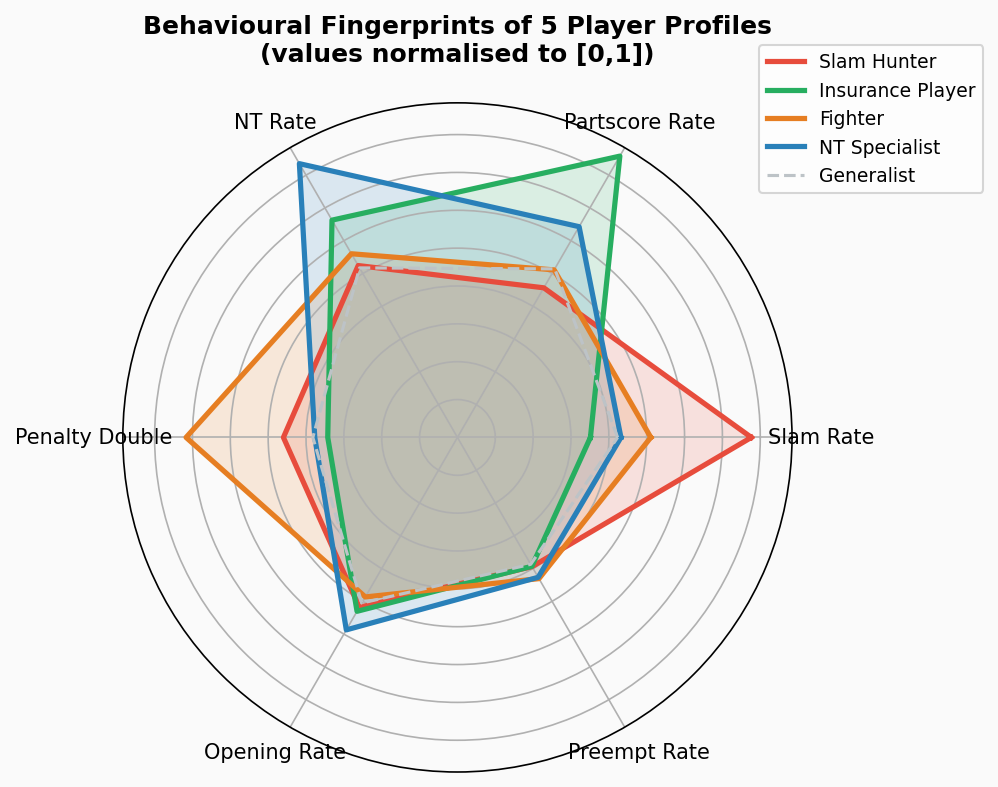
\includegraphics[width=0.78\textwidth]{radar_profiles.png}
\caption{Behavioral fingerprints of the four extreme profiles against
the Generalist baseline (all features z-scored). Each profile is extreme
on its own defining axis, and only mildly deviant elsewhere.}
\label{fig:radar}
\end{figure}

\paragraph{Known confounds (retained as limitations).} Bridge is a
partnership game: part of an elevated slam rate may reflect an
aggressive partner rather than the individual. The NT rate partly
reflects the pair's bidding system (e.g.\ Precision opens 1NT on wider
ranges). The Insurance Player signal is the weakest ($1.20\times$) and
may partly reflect hand-distribution variance. The Fighter is
methodologically the cleanest profile: doubling is a deliberate
individual act, its denominator counts both sides of the table, and its
base rate ($\sim$8.5\%) narrows confidence intervals quickly.

% ==================================================================
\section{Stage 2: Evidence-Grounded Skill Extraction}\label{sec:stage2}

For each profiled player we sample up to 50 boards (deterministic,
seed 42) and format them in chunks of 25 boards per LLM call. Each board
is rendered as four compact lines, showing the player's 13 cards, the full
auction with seats labeled, the final contract, and the numeric result:

\begin{quote}\small\ttfamily
Board 12 (Dealer N, Vul: NS)\\
You are S (Declarer). Your hand: $\spadesuit$AKQ74 $\heartsuit$A8 $\diamondsuit$KQ95 $\clubsuit$K3\\
Bidding: N:1D E:Pass S:1S W:Pass | N:3S E:Pass S:4NT W:Pass | N:5H E:Pass S:6S W:Pass ...\\
Result: 6S by S, made 12 tricks, NS +1430
\end{quote}

The extraction model (\texttt{gemini-2.5-flash}, temperature 0.3,
JSON-schema output) is instructed to act as a bridge expert and return 3--5
\emph{observable, falsifiable} skills, each with a name, a one-sentence
behavioral description, per-board evidence citations, and a confidence
grade; personality adjectives are explicitly forbidden. A
profile-context block deliberately directs the model's attention to the
profile's defining behavioral \emph{axis} (e.g.\ ``this player is in
the top decile of slam bidders; at least two skills must concern slam
bidding''); without such direction, rare defining behaviors drown under
generic competitive-bidding observations. The model never receives the
engineered feature values, the z-scores, or any comparative statistics:
everything it asserts must cite specific deals as evidence, and
Sec.~\ref{sec:validation} established, independently of any LLM, that
the directed-to behaviors are genuinely present in these players'
records. Whether downstream behavior follows skill content rather than
profile identity is tested separately by the inverse-prompt control
(Sec.~\ref{sec:control}).
Skills are aggregated across chunks and players into a per-profile
signature by TF--IDF cosine matching with a merge threshold of 0.40
(at 0.30, unrelated skills merged falsely; the threshold sweep is in the
repository). TF--IDF is preferred over neural embeddings deliberately:
at this scale (dozens of short, domain-specific skill names) lexical
overlap is the relevant signal, and the aggregation stays deterministic
and auditable, in line with the reproducibility goals. Typical extracted skills: \emph{``uses Roman Key Card
Blackwood to drive to slam with fitting hands''} (Slam Hunter);
\emph{``doubles opponents' partscores for penalty with trump stacks''}
(Fighter); \emph{``declines game invitations with borderline values''}
(Insurance Player).

This design carries the first half of the paper's anti-tautology
burden: the downstream agents are conditioned on \emph{what the player
demonstrably did with the cards}, not on adjectives we invented. The
second half, that agent behavior follows this content rather than the
profile's name, is carried by the inverse-prompt control
(Sec.~\ref{sec:control}).

% ==================================================================
\section{Stage 3: Profile-Conditioned Agents}\label{sec:stage3}

Each of the five agents (four profiles + Generalist control) is an LLM
(\texttt{gemini-2.5-flash}) with a system prompt assembled from: (i) an
identity line naming the profile and its one-line essence; (ii) the
Stage-2 skill list, the only content derived from the player's actual
record; (iii) domain rule constraints; and (iv) a mandatory JSON output
schema with a free-text rationale field. The identity line does name
the profile; whether measured behavior is driven by that name or by the
skill content is exactly what the inverse-prompt control of
Sec.~\ref{sec:control} tests, by swapping only the skills while leaving
every identity line in place. Bridge agents run at temperature 0.3
(later 0.0), negotiation agents at 0.7.

\paragraph{Mechanism check (one hand, five agents).} All five agents
received the same strong responding hand ($\spadesuit$AKQ72
$\heartsuit$AK4 $\diamondsuit$A83 $\clubsuit$Q2, 22 HCP) after partner
opened 1$\spadesuit$:

\begin{table}[h]
\centering\small
\caption{Same hand, five agents: the bid tracks the profile.}
\label{tab:samehand}
\begin{tabular}{lll}
\toprule
Agent & Bid & Rationale gist (agent's own output)\\
\midrule
Slam Hunter      & 4$\clubsuit$ & slam try; drives toward 6$\spadesuit$\\
Fighter          & 2NT (Jacoby) & game-force, keeps slam in view\\
NT Specialist    & 3NT          & prefers no-trump despite the fit\\
Generalist       & 3NT          & standard value bid, no slam push\\
Insurance Player & 4$\spadesuit$ & signs off in the safe game\\
\bottomrule
\end{tabular}
\end{table}

An expert pass over early outputs exposed bridge-mechanics errors
(a ``splinter'' announced on a doubleton; a 1NT overcall on 12 HCP). We
hardened the prompts with three rule blocks (convention correctness,
seat awareness, self-count of HCP) and re-ran: the mechanical errors
disappeared while profile-consistent choices persisted. Both prompt
versions are in the repository.

\paragraph{Reproducibility of LLM agents.} Even at temperature 0 the
API is not bit-reproducible (parallel floating-point reduction flips
borderline decisions). We therefore (a) persist every raw model output,
so all analyses are exactly reproducible from the archived JSON even if
regeneration differs; and (b) report distributions over many decisions,
never single calls. We flag this as a general methodological requirement
for LLM-agent experiments: \emph{sample-level, not call-level,
reproducibility}.

% ==================================================================
\section{Stage 4: Dual-Domain Evaluation}\label{sec:stage4}

Both domains use \emph{fixed, deterministic} counterparts, so that all
between-agent variation is attributable to the profiles.

\subsection{Bridge: metric falsification and a real-data skill measure}\label{sec:bridgemetric}

Our first bridge score rewarded bidding the level implied by combined
high-card points. We falsified it with a \textbf{ZI-C--style baseline}
in the spirit of Gode and Sunder's zero-intelligence constrained traders
\cite{gode1993zi}: a bidder drawing uniformly from the legal calls
\emph{beat the elite-derived agents} on this metric: the score
rewarded stating the formula, not making the contract. Any metric a
constrained random agent can top is broken; we discarded it.

The corrected measure uses the duplicate structure of the data itself
(no simulation). Every board is played at two tables; define the board
\emph{datum} as the cross-table mean score. A pair's skill on a board is
its score minus the datum, converted to IMPs (the official non-linear
scale that compresses extreme boards); player skill averages over a
player's boards, profile skill over its players. Defensive excellence, including successful penalty doubles, scores automatically. On
this scale the ZI-C bidder sits near $-7$ IMP/board, elite players near
$0$, and a double-dummy oracle \cite{ginsberg2001gib} at $+1.1$
(Fig.~\ref{fig:spectrum}); the metric now orders random $<$ human
$<$ omniscient, as any valid skill measure must.

\begin{figure}[t]
\centering
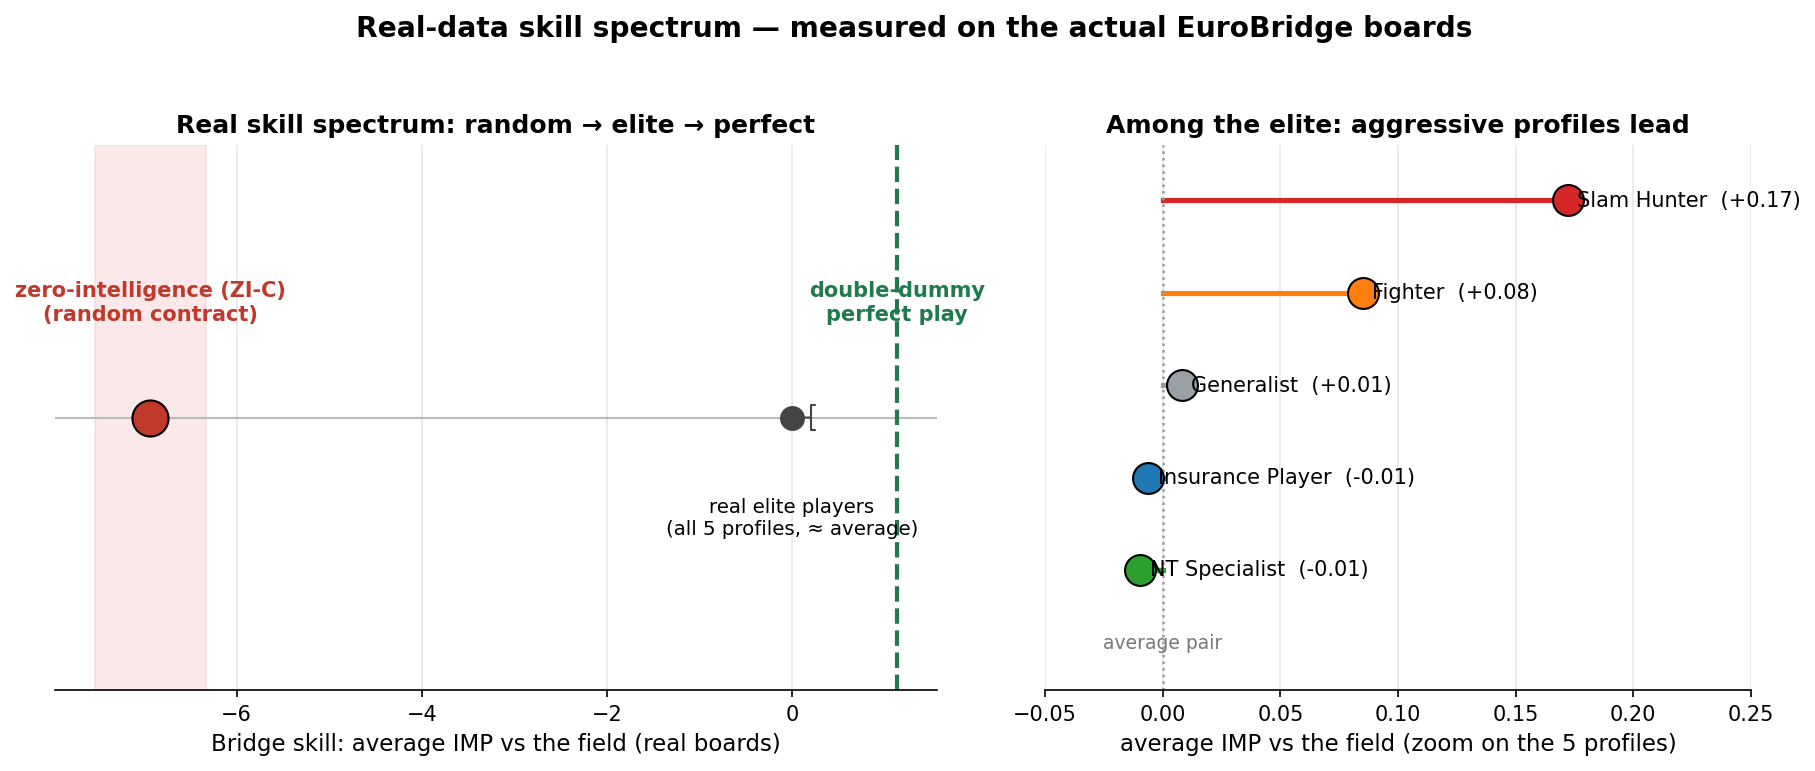
\includegraphics[width=0.8\textwidth]{real_skill_spectrum.png}
\caption{The validated skill spectrum: the ZI-C random baseline loses
$\sim$7 IMP/board to the field; elite profiles cluster near the datum;
the double-dummy oracle gains $+1.1$. A metric that cannot reproduce
this ordering is measuring the wrong thing.}
\label{fig:spectrum}
\end{figure}

\subsection{Negotiation: protocol, calibration, and a trivial example first}\label{sec:nego}

Each agent, acting as \emph{buyer}, negotiates four business scenarios (acquiring a SaaS startup; buying out a co-founder's equity; acquiring a competitor's customer book; and a multi-year enterprise licence), three runs each, against one fixed rule-based seller. The
seller opens at its ask $P_{\mathrm{ask}}$, accepts any offer
$\ge 0.95\,P_{\mathrm{ask}}$, otherwise concedes 15\% of the current gap
per round, never below its floor $P_{\mathrm{floor}}$, for at most 4
rounds; it walks away on the second ``absurd'' offer (below
$0.70\,P_{\mathrm{floor}}$). These constants are not free parameters:
they were calibrated on \textbf{5{,}247 human--human bargaining
dialogues} of the CraigslistBargain corpus \cite{he2018decoupling}: crowdsourced negotiations between people over real Craigslist listings (the corpus' training split; 6{,}682 dialogues in total, of which 4{,}334 carry usable price fields). In that corpus
aggressive lowballing captures more surplus while the deal rate barely
drops ($\approx0.83$ vs $0.86$): human sellers tolerate hard bargaining
and abandon only absurd offers. An
earlier, harsher walk-away rule reversed the results by punishing all
aggression; we document that sensitivity in
Sec.~\ref{sec:winning}. The negotiation outcome
is the \emph{surplus captured},
$\sigma = (P_{\mathrm{ask}}-P_{\mathrm{deal}})/
(P_{\mathrm{ask}}-P_{\mathrm{floor}})\in[0,1]$, zero if no deal. All
four scenarios are single-issue price negotiations, \emph{distributive} bargaining in the classical sense of Walton and
McKersie \cite{walton1965behavioral}; integrative, multi-issue scenarios
are deferred to future work (Sec.~\ref{sec:conclusion}).

Following the principle of trivial-first evaluation, note the reader can
predict this instrument's outcome: against a seller who concedes only
under pressure, aggressive anchor-low profiles should capture more
surplus, and cautious profiles should close early at worse prices.
Fig.~\ref{fig:nego} shows one real scenario: the aggressive profiles
anchor near the floor and hold; the cautious profiles drift up toward
the seller. The instrument behaves as expected, which is what
licenses its use on the non-trivial cross-domain question.

\begin{figure}[t]
\centering
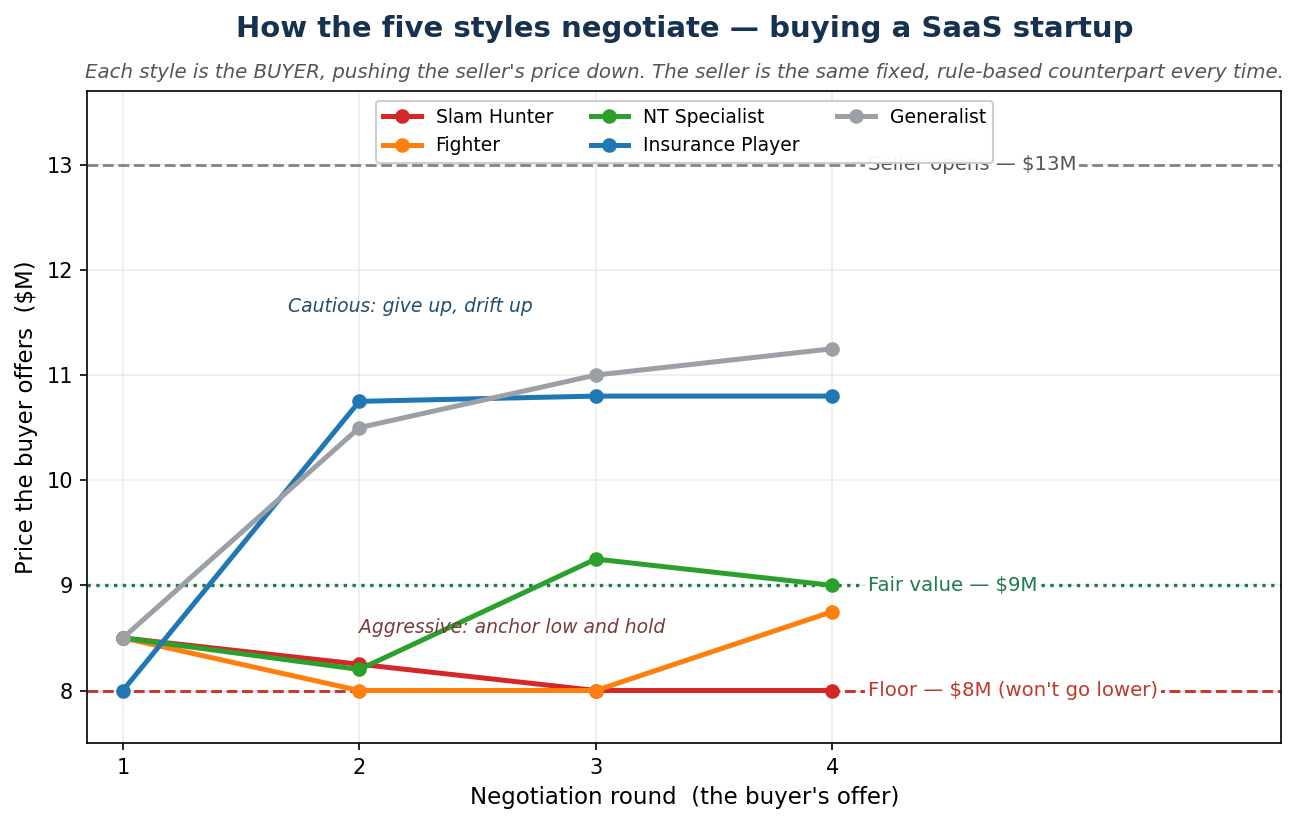
\includegraphics[width=0.85\textwidth]{negotiation_example.png}
\caption{One negotiation, five buyers (SaaS scenario: ask \$13M, fair
value \$9M, floor \$8M; real run-0 offer trajectories). Aggressive
bridge profiles anchor low and hold; cautious profiles concede upward.}
\label{fig:nego}
\end{figure}

% ==================================================================
\section{Implementation and Software Engineering}\label{sec:engineering}

The pipeline is engineered as a single research software product rather
than a collection of scripts, a choice worth stating explicitly given
this volume's software-tools theme. All public operations flow through
one SDK entry point (\texttt{src/sdk.py}); no function lives only in a
notebook. LLM access is routed through a provider-agnostic client
(\texttt{src/shared/llm\_client.py}) that logs model, token counts,
latency, and cost for every call and enforces a budget guard (alert at
\$20, hard cap at \$50); swapping the model provider is a one-argument
change, which is how the cross-provider replication planned as future
work is already wired. The code is typed, linted, and documented, with
data hygiene enforced by convention: raw inputs are read-only, and all
derived artifacts live under separate processed and results trees. A
pytest suite of 178 tests covers the feature engineering, the profiling
gates, the statistical validators, and the agents; LLM-dependent
components are tested by injecting a mocked client, so the full suite
runs without network access or cost. These practices are what make the
reproduction protocol of Appendix~\ref{app:protocol} executable by a
stranger rather than aspirational.

% ==================================================================
\section{Results}\label{sec:results}

\subsection{Winning does not transfer cleanly}\label{sec:winning}

We first correlated per-profile \emph{winning} in bridge with winning in
negotiation (Spearman rank correlation over the $K=5$ profiles). The
answer depends on the bridge metric
(Table~\ref{tab:sensitivity}): the discarded par-proxy gives
$\rhoS=+0.30$; a fight-aware blend rises monotonically with the weight
on doubling; the validated real-data IMP metric gives $\rhoS=+0.20$,
with $+0.50$ under a raw-points robustness variant. With
$K=5$, none is significant.

\begin{table}[h]
\centering\small
\caption{Winning$\leftrightarrow$winning is metric-sensitive.
The final row is the validated metric of Sec.~\ref{sec:bridgemetric}.}
\label{tab:sensitivity}
\begin{tabular}{lc}
\toprule
Bridge-side metric & $\rhoS$ (win vs.\ win, $K=5$)\\
\midrule
Par-level proxy (falsified by ZI-C) & $+0.30$\\
Fight-aware blend, weight $w=0.2 / 0.3 / 0.4$ & $+0.60\; /\; +0.70\; /\; +0.90$\\
Real-data IMP-vs-datum (validated) & $\mathbf{+0.20}$\\
\bottomrule
\end{tabular}
\end{table}

We read this as a substantive lesson, not a failure: \emph{whether a
style wins depends on the opponent and the payoff rules}: an over-harsh seller inverted the sign entirely in one ablation, so
winning$\leftrightarrow$winning is the wrong invariant to chase across
domains.

\subsection{Style transfers: behavioral alignment $\rhoS = +0.80$}\label{sec:style}

The research question was always \emph{behavioral} alignment. Define
bridge-side aggression of a profile as the mean composite z-score of its
members on the three action axes
$\{$\texttt{slam\_rate}, \texttt{preempt\_rate},
\texttt{penalty\_double\_rate}$\}$, and negotiation-side aggression as
\emph{demand depth}: how far below the ask the agent's opening offer
reaches,
\begin{equation}
\theta \;=\; \frac{P_{\mathrm{ask}} - P_{\mathrm{open}}^{\mathrm{buyer}}}
{P_{\mathrm{ask}} - P_{\mathrm{floor}}}\;,
\label{eq:theta}
\end{equation}
averaged over scenarios and runs (from the archived logs; no new
simulation). Demand depth operationalizes first-offer aggressiveness,
whose anchoring effect on negotiation outcomes is well documented
\cite{galinsky2001first}.

\begin{table}[h]
\centering\small
\caption{Style$\leftrightarrow$style alignment across domains.}
\label{tab:style}
\begin{tabular}{lcc}
\toprule
Profile & Bridge aggression (z) & Negotiation demand depth $\theta$\\
\midrule
Fighter          & $+1.30$ & 0.808\\
Slam Hunter      & $+0.51$ & 0.760\\
NT Specialist    & $-0.36$ & 0.771\\
Generalist       & $-0.69$ & 0.666\\
Insurance Player & $-0.77$ & 0.666\\
\midrule
\multicolumn{3}{c}{Spearman $\rhoS = \mathbf{+0.80}$ \; (two-sided $p=0.10$, $K=5$)}\\
\bottomrule
\end{tabular}
\end{table}

Aggressive bridge profiles bargain aggressively; cautious ones bargain
softly (Fig.~\ref{fig:style}). The one rank inversion (NT Specialist
above Slam Hunter on $\theta$) is what caps $\rhoS$ at $0.80$ rather than $1.0$; this is expected, since the NT axis is stylistic rather than
directly risk-graded.

A note on inference is due here rather than in the limitations. With
$K=5$, the permutation null admits only $5!=120$ orderings, so the
smallest attainable two-sided $p$ is $0.017$, and only near-perfect
rankings ($|\rhoS|\ge0.9$) clear the conventional $0.05$ threshold; the
observed $+0.80$ sits exactly one adjacent rank swap short of that, at
$p=0.10$. We therefore make no significance claim for the alignment
itself and read $+0.80$ as an effect-size indication whose inferential
support comes from converging evidence: the profile foundations are
individually significant (Table~\ref{tab:cohend}, and every assignment
gate of Eq.~\ref{eq:gate} holds at $p<0.05$), and the inverse-prompt
control (Sec.~\ref{sec:control}) is nominally significant on its own
($p=0.037$).

\begin{figure}[t]
\centering
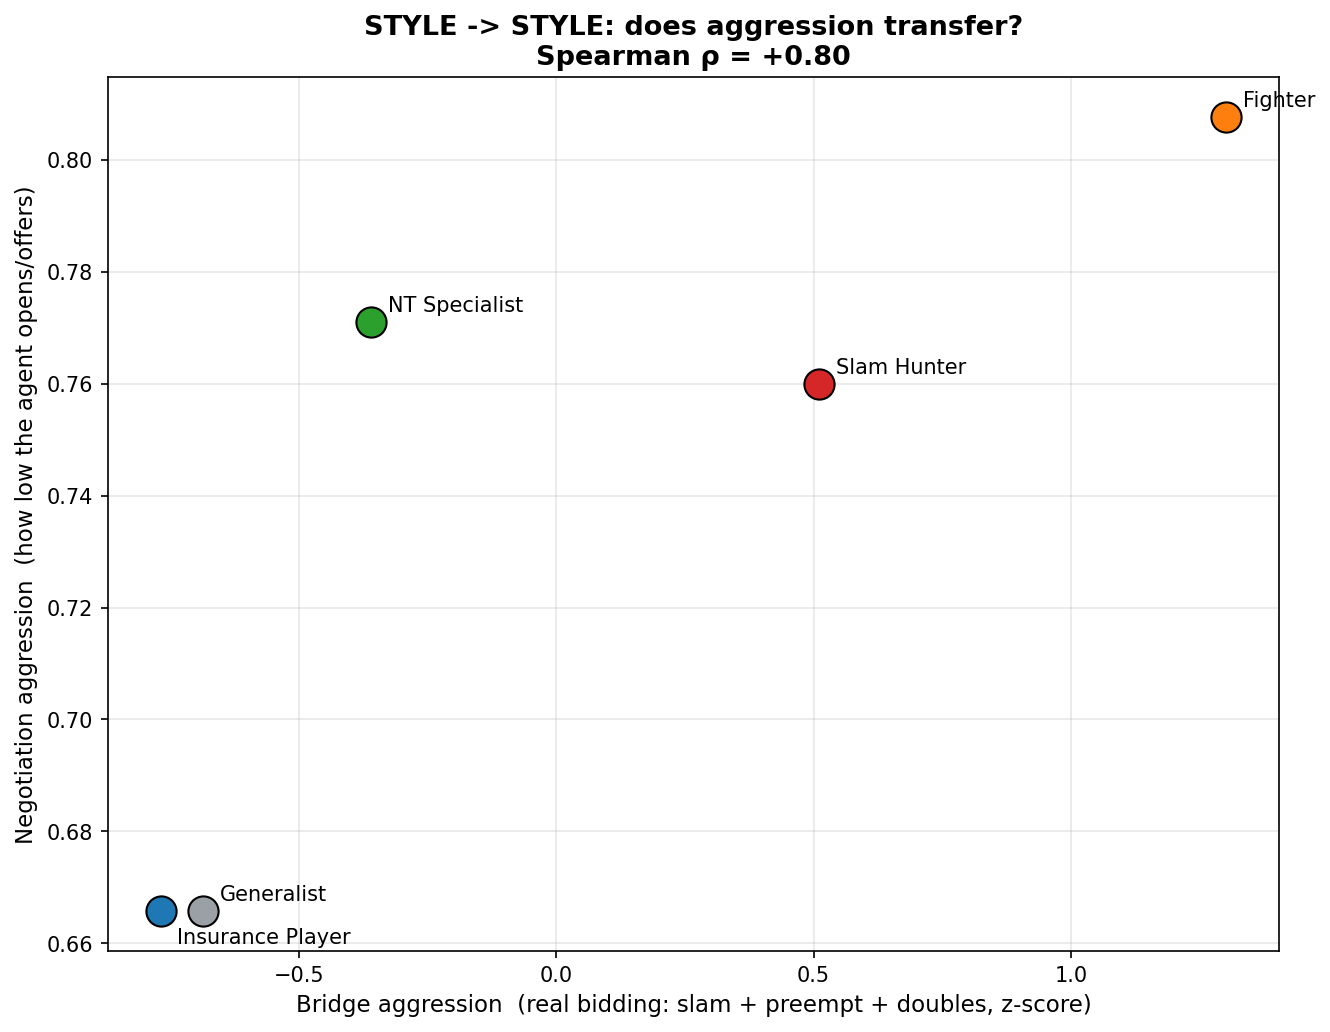
\includegraphics[width=0.8\textwidth]{style_alignment.png}
\caption{Behavioral alignment: bridge-derived aggression (x) vs.\
negotiation demand depth (y), $\rhoS=+0.80$.}
\label{fig:style}
\end{figure}

\subsection{The inverse-prompt control: $\rhoS = -0.90$}\label{sec:control}

Could the agents simply be acting out their names? Control: keep every
identity line intact but inject the \emph{opposite} profile's Stage-2
skills (Fighter gets the Insurance skill list and vice versa), then
re-measure $\theta$. If behavior follows the label, nothing should
change; if it follows the skills, the correlation should invert. It
inverts: the Fighter with Insurance skills softens
($\theta: 0.808\to0.725$), the Insurance Player with Fighter skills
hardens ($0.666\to0.805$), and the cross-domain correlation flips to
$\rhoS=\mathbf{-0.90}$ (two-sided $p=0.037$; Fig.~\ref{fig:control}). The
$+0.80$ alignment is therefore \emph{skill-mediated}: it is carried by
behavior extracted from real hands, not by the profile's name.

\begin{figure}[t]
\centering
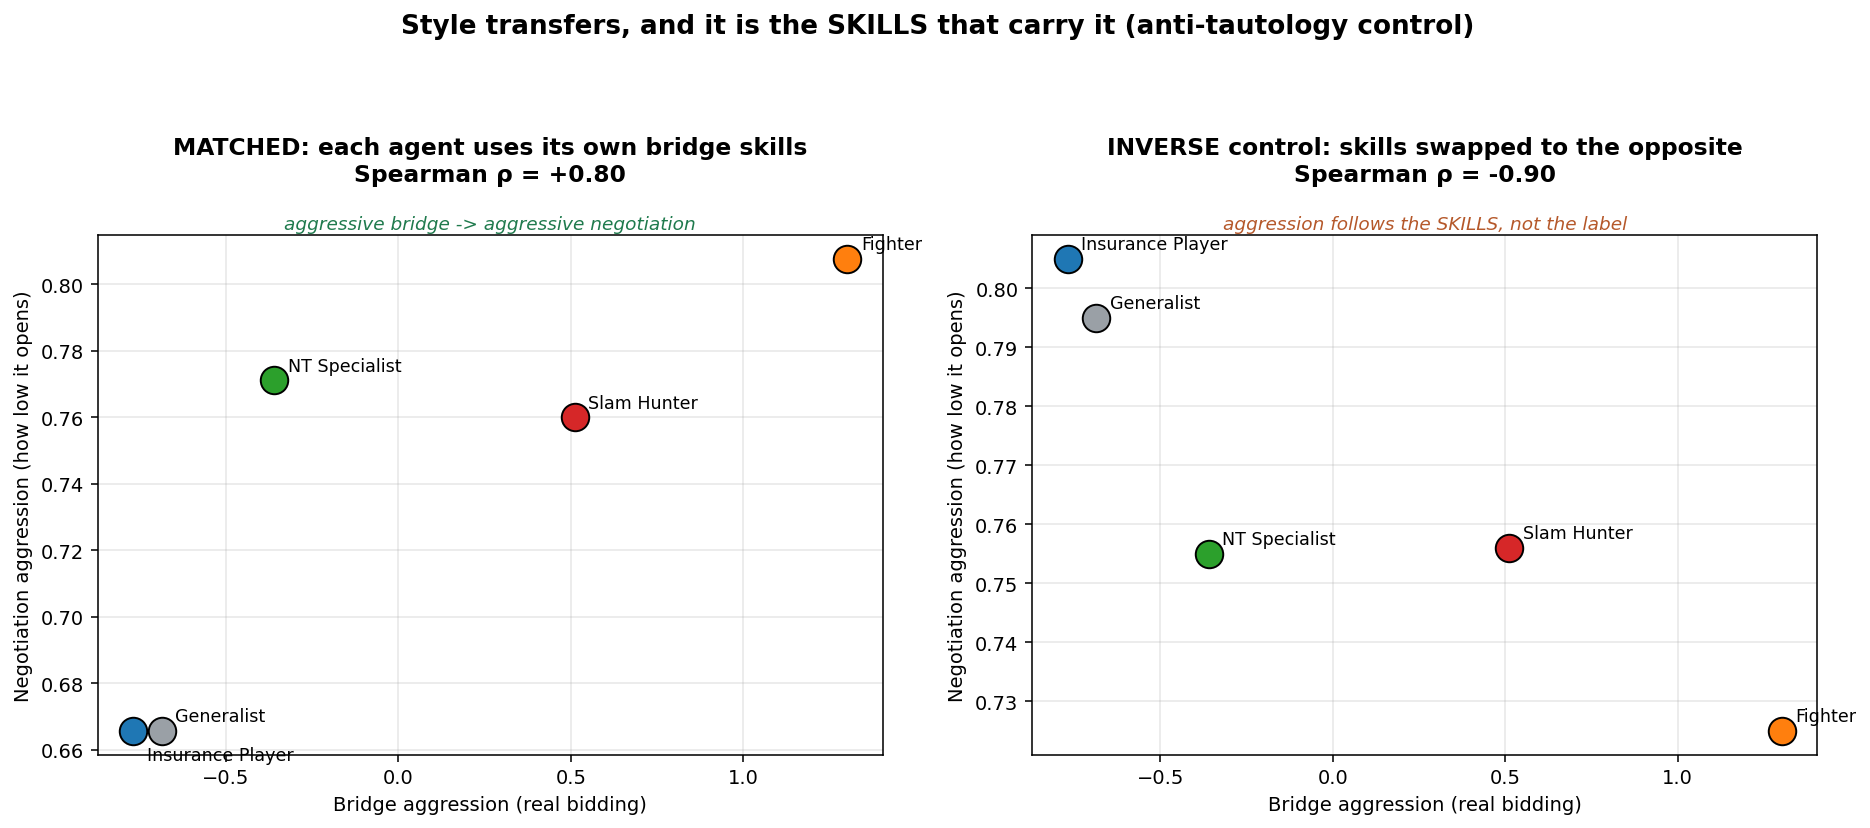
\includegraphics[width=0.8\textwidth]{style_transfer_control.png}
\caption{Inverse-prompt control. Swapping each profile's bridge-derived
skills (labels unchanged) flips the alignment from $+0.80$ to $-0.90$:
the behavior follows the skills, not the label.}
\label{fig:control}
\end{figure}

% ==================================================================
\section{Discussion}\label{sec:discussion}

\paragraph{Reading the pair of results.} The two findings are two sides
of one coin. Decision \emph{style}, how much risk you demand and how hard you hold a position, is a property of the decision-maker and survives
domain transfer ($+0.80$, controlled). \emph{Winning} is a property of
the decision-maker \emph{jointly with} the environment's payoff
structure and counterpart, and does not transfer stably ($+0.2$ to
$+0.5$, sign-reversible under an unrealistic counterpart). In
optimization terms: the agents carry a stable preference structure over
the risk--reward trade-off into a new decision problem, while the
\emph{value} of that preference structure depends on the objective
landscape it meets. This distinction matters practically: profiling a
counterpart's style from observable past behavior is feasible and
predictive of \emph{how} they will negotiate, not necessarily of who
wins.

\paragraph{Methodological exports.} Three components are reusable beyond
bridge: (i) the significance-gated tail-profiling recipe for
low-base-rate behaviors (Eq.~\ref{eq:gate}); (ii) metric falsification
by constrained-random baseline (a ZI-C agent must rank last, an oracle
first) before any cross-domain claim; (iii) evidence-grounded skill
extraction plus an inverse-prompt control as an anti-tautology standard
for LLM-persona experiments.

\paragraph{Limitations.} With $K=5$ profiles, only near-perfect rank
orderings ($|\rhoS|\ge0.9$) can clear $p<0.05$
(Sec.~\ref{sec:style}); the observed alignment ($p=0.10$) is therefore
an indication, and scaling the number of profiles (finer tail slices,
per-player agents) is the direct fix. The negotiation domain is
simulated: the counterpart is rule-based (though data-calibrated), the
scenarios are single-issue price negotiations, and surplus is the sole
outcome. Bridge-side confounds remain (partnership effects on
\texttt{slam\_rate}; convention systems on \texttt{nt\_rate}). The skill
extractor and the agents share one model family (Gemini), so
provider-specific behavior cannot yet be ruled out; the
provider-agnostic client of Sec.~\ref{sec:engineering} makes
cross-provider replication (Claude, GPT) a one-argument change, and it
is the first robustness item of future work. Finally,
elite players are a selected population; transfer from amateur play is
untested.

% ==================================================================
\section{Conclusions and Future Work}\label{sec:conclusion}

We built and validated, end to end, a reproducible pipeline that turns
149{,}208 real tournament records into statistically gated
decision-making profiles, disentangles their behavioral content from
their labels, instantiates them as LLM agents, and measures their
behavior in a second, unrelated domain. The empirical yield: elite
decision styles form a continuum whose tails are behaviorally real
(Cohen's $d$ 2.1--4.6); their \emph{style} persists across domains
($\rhoS=+0.80$; inverse control $-0.90$); their \emph{success} does not
persist cleanly ($\rhoS\approx+0.2$ to $+0.5$).

Three extensions are planned. \emph{Team negotiations:} multi-agent
teams mixing profiles (e.g.\ a Fighter--Insurance buying team) to study
intra-team dynamics, bridging to coalition and alliance formation.
\emph{Multi-stage deals:} a memorandum-of-understanding phase followed
by substantive bargaining, testing whether style expression differs by
phase. \emph{Multi-criteria negotiation:} price plus quality plus
optional features, which recasts the interaction as a multiobjective
optimization problem with heterogeneous preference structures, and connects directly to interactive multiobjective decision support.
On the bridge side, the natural deepening is a learned
estimation--policy architecture (ENN/PNN \cite{rong2019bridge}) over the
full corpus, and per-player (rather than per-profile) agents to raise
$K$ from 5 to hundreds. On the negotiation side, future work targets
real human negotiation data. A concrete first step is the CaSiNo corpus
\cite{chawla2021casino}: 1{,}030 multi-issue human negotiations in
which each negotiator carries measured Big-Five and social-value-orientation scores: exactly the trait$\to$behavior linkage this paper constructs
synthetically, now testable on humans (does measured trait-level
aggression predict human demand depth the way bridge-derived profiles
predict it in agents?). Its integrative, three-issue structure also
supplies the multi-criteria scenarios for the extension above, closing
the loop the laboratory opened.

% ==================================================================
\section*{Reproducibility Statement}\label{sec:repro}

All code, prompts, thresholds, seeds, and archived model outputs are at
\url{https://github.com/annafr2/From-Bridge-Tables-to-Global-Markets}.
Fixed constants: qualification $n\ge50$ declared and $\ge50$ bidding
boards; percentile gate top 10\%; binomial gate $\alpha=0.05$
(one-sided, SciPy \texttt{binomtest} \cite{virtanen2020scipy});
cv-filter $0.10$; K-Means/GMM/HDBSCAN via scikit-learn
\cite{pedregosa2011scikit} with \texttt{random\_state}=42; LLM chunking
25 boards/call, $\le50$ boards/player, sampling seed 42; skill-merge
TF--IDF threshold 0.40; temperatures 0.3 (extraction), 0.3/0.0 (bridge),
0.7 (negotiation); seller rule: accept $\ge0.95\,P_{\mathrm{ask}}$,
concede 15\% of gap/round, floor-bounded, $\le4$ rounds, walk-away after
2 offers below $0.70\,P_{\mathrm{floor}}$. Result-to-script map: profiles (\texttt{src/stage1\_clustering/}); audit (\texttt{notebooks/preprocessing\_comparison.py}); validation (\texttt{notebooks/validate\_base\_rates.py}); skill spectrum and metrics (\texttt{notebooks/alignment\_real\_bridge.py}, \texttt{visualize\_real\_skill\_spectrum.py}); style alignment and control (\texttt{notebooks/style\_alignment.py}, \texttt{inverse\_prompt\_control.py}); negotiation calibration (\texttt{notebooks/validate\_negotiation\_features.py}). Environment:
Python~3.11; scikit-learn, SciPy~1.11, pandas (versions pinned in
\texttt{requirements.txt}); all LLM stages use
\texttt{gemini-2.5-flash} through a single provider-agnostic client.
Every LLM call is logged with model, token counts, and cost (total
compute cost of all experiments: under \$10).
Appendix~\ref{app:protocol} gives the numbered, end-to-end reproduction
protocol.

\section*{Acknowledgments}

The author thanks Prof.\ Jari H\"am\"al\"ainen and Prof.\ Pekka
Neittaanm\"aki (LUT University) for doctoral supervision and for
guidance on the scientific framing of this work; Dr.\ Nezer Jacob
Zaidenberg for bridge-domain expert review that materially improved the
profiling methodology (Sec.~\ref{sec:profiles}); and Dr.\ Yoram Segal
for the engineering-first project framework within which the system was
built. Generative AI tools (Google Gemini, Anthropic Claude) are the
object of study in Stages 2--4 and were additionally used for language
polishing and as coding assistants; all scientific content, design
choices, analyses, and conclusions are the author's own.

% ==================================================================
\appendix
\section{Step-by-Step Reproduction Protocol}\label{app:protocol}

The protocol below reproduces every table and figure in this paper.
Steps 1--5 are fully deterministic (no API key, no cost). Steps 6--7
and 10 call the LLM and are therefore \emph{distributionally}
reproducible (Sec.~\ref{sec:stage3}); the raw model outputs of our runs
ship in the repository, so steps 8--9 and 11 can be reproduced
\emph{exactly} from the archive without re-querying any model.

\begin{enumerate}
  \item \textbf{Environment.} Clone
  \url{https://github.com/annafr2/From-Bridge-Tables-to-Global-Markets};
  create a Python~3.11 virtual environment; \texttt{pip install -r
  requirements.txt}. For steps 6--7 only, set \texttt{GOOGLE\_API\_KEY}
  in \texttt{.env}.
  \item \textbf{Data check.} Load the corpus via
  \texttt{src/shared/data\_loader.py}. Expected: 149{,}208 board-room
  records; per-championship coverage as in Table~\ref{tab:data}.
  \item \textbf{Stage 1: features and profiles.} Run the Stage-1
  pipeline (\texttt{src/stage1\_clustering/}: \texttt{features.py} with
  \texttt{MIN\_BOARDS}=50, then \texttt{extreme\_profiles.py} with
  top-10\% cutoff and $\alpha=0.05$). Expected output:
  \texttt{data/processed/player\_profiles.csv} with 563 rows and profile
  counts 20/21/37/17/468 (Table~\ref{tab:profiles}).
  \item \textbf{Cluster-structure audit.} \texttt{python -m
  notebooks.preprocessing\_comparison}. Expected: the five
  configurations of Table~\ref{tab:audit} (max silhouette 0.24; HDBSCAN
  0 clusters) and \texttt{results/preprocessing.xlsx}.
  \item \textbf{Profile validation.} \texttt{python -m
  notebooks.validate\_base\_rates}. Expected: the effect sizes and
  $p$-values of Table~\ref{tab:cohend}.
  \item \textbf{Stage 2: skill extraction} (LLM; $\approx$\$1). Run
  the extractor over all profiled players
  (\texttt{src/stage2\_skills/}; chunks of 25 boards, $\le$50
  boards/player, sampling seed 42, temperature 0.3,
  \texttt{gemini-2.5-flash}); aggregate with TF--IDF merge threshold
  0.40. Output: the per-profile skill signatures JSON.
  \item \textbf{Stages 3--4: dual-domain simulation} (LLM;
  $<$\$5). \texttt{python -m src.stage4\_simulate.bridge\_runner} and
  \texttt{python -m src.stage4\_simulate.negotiation}. All raw agent
  outputs are persisted under \texttt{results/stage4/}.
  \item \textbf{Bridge skill metric and spectrum.} \texttt{python -m
  notebooks.alignment\_real\_bridge} and \texttt{python -m
  notebooks.visualize\_real\_skill\_spectrum}. Expected:
  Fig.~\ref{fig:spectrum} and the win--win row of
  Table~\ref{tab:sensitivity} ($\rhoS=+0.20$ on IMPs, $+0.50$ on raw
  points).
  \item \textbf{Style alignment.} \texttt{python -m
  notebooks.style\_alignment}, recomputed from the archived Stage-4
  logs with no new simulation. Expected, \emph{exactly}:
  Table~\ref{tab:style} and Fig.~\ref{fig:style} ($\rhoS=+0.80$).
  \item \textbf{Inverse-prompt control} (LLM; $<$\$1). \texttt{python
  -m notebooks.inverse\_prompt\_control} re-runs the swapped-skill
  negotiations with live model calls, so it reproduces
  distributionally; the archived outputs behind Fig.~\ref{fig:control}
  ($\rhoS=-0.90$) ship in the repository.
  \item \textbf{Seller calibration.} \texttt{python -m
  notebooks.validate\_negotiation\_features} against the
  CraigslistBargain training split under \texttt{data/external/}.
  Expected: 4{,}334 usable dialogues; aggressive opening captures more
  surplus at a deal rate of $\approx0.83$ vs $0.86$
  (Sec.~\ref{sec:nego}).
\end{enumerate}

% ==================================================================
\begin{thebibliography}{99}\small

\bibitem{ginsberg2001gib}
Ginsberg, M.\,L.:
GIB: Imperfect information in a computationally challenging game.
Journal of Artificial Intelligence Research \textbf{14}, 303--358 (2001)

\bibitem{rong2019bridge}
Rong, J., Qin, T., An, B.:
Competitive bridge bidding with deep neural networks.
arXiv preprint arXiv:1903.00900 (2019)

\bibitem{silver2018general}
Silver, D., et al.:
A general reinforcement learning algorithm that masters chess, shogi,
and Go through self-play.
Science \textbf{362}(6419), 1140--1144 (2018)

\bibitem{kramar2022negotiation}
Kram\'ar, J., et al.:
Negotiation and honesty in artificial intelligence methods for the
board game of Diplomacy.
Nature Communications \textbf{13}, 7214 (2022)

\bibitem{bakhtin2022cicero}
Meta Fundamental AI Research Diplomacy Team (FAIR), Bakhtin, A., et al.:
Human-level play in the game of Diplomacy by combining language models
with strategic reasoning.
Science \textbf{378}(6624), 1067--1074 (2022)

\bibitem{lewis2017deal}
Lewis, M., Yarats, D., Dauphin, Y., Parikh, D., Batra, D.:
Deal or no deal? End-to-end learning of negotiation dialogues.
In: Proc.\ EMNLP 2017, pp.~2443--2453 (2017)

\bibitem{he2018decoupling}
He, H., Chen, D., Balakrishnan, A., Liang, P.:
Decoupling strategy and generation in negotiation dialogues.
In: Proc.\ EMNLP 2018, pp.~2333--2343 (2018)

\bibitem{vaccaro2026advancing}
Vaccaro, M., Caosun, M., Ju, H., Aral, S., Curhan, J.\,R.:
Advancing AI negotiations: A large-scale autonomous negotiation
competition.
Proceedings of the National Academy of Sciences \textbf{123}(23),
e2521774123 (2026)

\bibitem{bianchi2024negotiationarena}
Bianchi, F., Chia, P.\,J., Yuksekgonul, M., Tagliabue, J., Jurafsky, D.,
Zou, J.:
How well can LLMs negotiate? NegotiationArena platform and analysis.
In: Proc.\ ICML 2024 (2024)

\bibitem{abdelnabi2024cooperation}
Abdelnabi, S., Gomaa, A., Sivaprasad, S., Sch\"onherr, L., Fritz, M.:
Cooperation, competition, and maliciousness: LLM-stakeholders
interactive negotiation.
In: Proc.\ NeurIPS 2024, Datasets and Benchmarks Track (2024)

\bibitem{chawla2021casino}
Chawla, K., Ramirez, J., Clever, R., Lucas, G., May, J., Gratch, J.:
CaSiNo: A corpus of campsite negotiation dialogues for automatic
negotiation systems.
In: Proc.\ NAACL 2021, pp.~3167--3185 (2021)

\bibitem{mannekote2025roleplaying}
Mannekote, A., Davies, A., Li, G., Boyer, K.\,E., Zhai, C., Dorr, B.\,J.,
Pinto, F.:
Do role-playing agents practice what they preach? Belief-behavior
consistency in LLM-based simulations of human trust.
arXiv preprint arXiv:2507.02197 (2025)

\bibitem{gode1993zi}
Gode, D.\,K., Sunder, S.:
Allocative efficiency of markets with zero-intelligence traders: Market
as a partial substitute for individual rationality.
Journal of Political Economy \textbf{101}(1), 119--137 (1993)

\bibitem{kahneman1979prospect}
Kahneman, D., Tversky, A.:
Prospect theory: An analysis of decision under risk.
Econometrica \textbf{47}(2), 263--291 (1979)

\bibitem{cutler1994archetypal}
Cutler, A., Breiman, L.:
Archetypal analysis.
Technometrics \textbf{36}(4), 338--347 (1994)

\bibitem{brandenburger1996coopetition}
Brandenburger, A.\,M., Nalebuff, B.\,J.:
Co-opetition.
Currency Doubleday, New York (1996)

\bibitem{raiffa1982art}
Raiffa, H.:
The Art and Science of Negotiation.
Harvard University Press, Cambridge, MA (1982)

\bibitem{nash1950bargaining}
Nash, J.\,F.:
The bargaining problem.
Econometrica \textbf{18}(2), 155--162 (1950)

\bibitem{shoham2008multiagent}
Shoham, Y., Leyton-Brown, K.:
Multiagent Systems: Algorithmic, Game-Theoretic, and Logical
Foundations.
Cambridge University Press (2008)

\bibitem{rousseeuw1987silhouettes}
Rousseeuw, P.\,J.:
Silhouettes: A graphical aid to the interpretation and validation of
cluster analysis.
Journal of Computational and Applied Mathematics \textbf{20}, 53--65
(1987)

\bibitem{campello2013density}
Campello, R.\,J.\,G.\,B., Moulavi, D., Sander, J.:
Density-based clustering based on hierarchical density estimates.
In: Proc.\ PAKDD 2013, LNCS 7819, pp.~160--172. Springer (2013)

\bibitem{cohen1988statistical}
Cohen, J.:
Statistical Power Analysis for the Behavioral Sciences, 2nd edn.
Lawrence Erlbaum Associates, Hillsdale, NJ (1988)

\bibitem{mann1947test}
Mann, H.\,B., Whitney, D.\,R.:
On a test of whether one of two random variables is stochastically
larger than the other.
Annals of Mathematical Statistics \textbf{18}(1), 50--60 (1947)

\bibitem{spearman1904proof}
Spearman, C.:
The proof and measurement of association between two things.
American Journal of Psychology \textbf{15}(1), 72--101 (1904)

\bibitem{ericsson1996expert}
Ericsson, K.\,A., Lehmann, A.\,C.:
Expert and exceptional performance: Evidence of maximal adaptation to
task constraints.
Annual Review of Psychology \textbf{47}, 273--305 (1996)

\bibitem{park2023generative}
Park, J.\,S., O'Brien, J., Cai, C.\,J., Morris, M.\,R., Liang, P.,
Bernstein, M.\,S.:
Generative agents: Interactive simulacra of human behavior.
In: Proc.\ UIST 2023 (2023)

\bibitem{argyle2023out}
Argyle, L.\,P., Busby, E.\,C., Fulda, N., Gubler, J.\,R., Rytting, C.,
Wingate, D.:
Out of one, many: Using language models to simulate human samples.
Political Analysis \textbf{31}(3), 337--351 (2023)

\bibitem{aher2023using}
Aher, G., Arriaga, R.\,I., Kalai, A.\,T.:
Using large language models to simulate multiple humans and replicate
human subject studies.
In: Proc.\ ICML 2023 (2023)

\bibitem{virtanen2020scipy}
Virtanen, P., et al.:
SciPy 1.0: Fundamental algorithms for scientific computing in Python.
Nature Methods \textbf{17}, 261--272 (2020)

\bibitem{pedregosa2011scikit}
Pedregosa, F., et al.:
Scikit-learn: Machine learning in Python.
Journal of Machine Learning Research \textbf{12}, 2825--2830 (2011)

\bibitem{epstein1979stability}
Epstein, S.:
The stability of behavior: I. On predicting most of the people much of
the time.
Journal of Personality and Social Psychology \textbf{37}(7), 1097--1126
(1979)

\bibitem{mischel1995cognitive}
Mischel, W., Shoda, Y.:
A cognitive-affective system theory of personality: Reconceptualizing
situations, dispositions, dynamics, and invariance in personality
structure.
Psychological Review \textbf{102}(2), 246--268 (1995)

\bibitem{weber2002domain}
Weber, E.\,U., Blais, A.-R., Betz, N.\,E.:
A domain-specific risk-attitude scale: Measuring risk perceptions and
risk behaviors.
Journal of Behavioral Decision Making \textbf{15}(4), 263--290 (2002)

\bibitem{galinsky2001first}
Galinsky, A.\,D., Mussweiler, T.:
First offers as anchors: The role of perspective-taking and negotiator
focus.
Journal of Personality and Social Psychology \textbf{81}(4), 657--669
(2001)

\bibitem{walton1965behavioral}
Walton, R.\,E., McKersie, R.\,B.:
A Behavioral Theory of Labor Negotiations: An Analysis of a Social
Interaction System.
McGraw-Hill, New York (1965)

\bibitem{lloyd1982least}
Lloyd, S.\,P.:
Least squares quantization in PCM.
IEEE Transactions on Information Theory \textbf{28}(2), 129--137 (1982)

\bibitem{schwarz1978estimating}
Schwarz, G.:
Estimating the dimension of a model.
Annals of Statistics \textbf{6}(2), 461--464 (1978)

\bibitem{jolliffe2002principal}
Jolliffe, I.\,T.:
Principal Component Analysis, 2nd edn.
Springer, New York (2002)

\bibitem{clopper1934use}
Clopper, C.\,J., Pearson, E.\,S.:
The use of confidence or fiducial limits illustrated in the case of the
binomial.
Biometrika \textbf{26}(4), 404--413 (1934)

\end{thebibliography}

\end{document}
